\documentclass[11pt]{article}

\usepackage{latexsym}
\usepackage{amsmath}
\usepackage{amssymb}
\usepackage{amsthm}
\usepackage{graphicx}
\usepackage{wrapfig}
\usepackage{pseudocode}
\usepackage{url}
\usepackage[backref, colorlinks=true, citecolor=red, urlcolor=blue, pdfauthor={Jyh-Ming Lien}]{hyperref}
\usepackage{tabu}


\newcommand{\handout}[5]{
  \noindent
  \begin{center}
  \framebox{
    \vbox{
      \hbox to 5.78in { {\bf } \hfill #2 }
      \vspace{4mm}
      \hbox to 5.78in { {\Large \hfill #5  \hfill} }
      \vspace{2mm}
      \hbox to 5.78in { {\em #3 \hfill #4} }
    }
  }
  \end{center}
  \vspace*{4mm}
}

\newcommand{\lecture}[4]{\handout{#1}{#2}{#3}{#4}{#1}}

\newtheorem{theorem}{Theorem}
\newtheorem{corollary}[theorem]{Corollary}
\newtheorem{lemma}[theorem]{Lemma}
\newtheorem{observation}[theorem]{Observation}
\newtheorem{proposition}[theorem]{Proposition}
\newtheorem{definition}[theorem]{Definition}
\newtheorem{claim}[theorem]{Claim}
\newtheorem{fact}[theorem]{Fact}
\newtheorem{assumption}[theorem]{Assumption}

% 1-inch margins, from fullpage.sty by H.Partl, Version 2, Dec. 15, 1988.
\topmargin 0pt
\advance \topmargin by -\headheight
\advance \topmargin by -\headsep
\textheight 8.9in
\oddsidemargin 0pt
\evensidemargin \oddsidemargin
\marginparwidth 0.5in
\textwidth 6.5in

\parindent 0in
\parskip 1.5ex
%\renewcommand{\baselinestretch}{1.25}

\begin{document}

\lecture{Midterm Exam Report}{Fall 2015}{Moran Kim}{Advance Algorithm Programming}

\section{Summary of the two methods}

\indent The two stippling methods are based on the same stroy. But the implementations are a little bit different. In this part, I will summarize these two methods.


\subsection{hedcuter method}
Given input N, which means the number of points in the image. The [Hedcut::sample$\_$initial$\_$points] function generates
N number of points which are evenly distributed in a black region. The positions of N number of sampled points are different since in sampling process the 'current time' is considered. As these N number of points are set as sites, the [CVT::vor] function computes the voronoi diagram. And to calculate the centroid of each voronoi cell later, all the points in the image are stored by its cell's sites. The sites are listed in [rootid] order and all the points of the images are stored in each cell(i.e. coverage). After collecting cells to compute the centroid voronoi diagram, we need to compute the centroid in each cell and move the sites to the centroid. This procedure can be described as, first compute the voronoi diagram and then compute the centroid, this two process will iterate until the maximum distance of the movements of the sites are less than that of given tolerance(in my case, 1).
\indent After computing the centroid of the voronoi diagram to make a stippling, the [Hedcut::create$\_$disks] function creates disks with the different sizes, depending on the cells size.(As the points brighter it has wider cell.) As the cell is bigger the color intensity of the centroid of that cell is smaller. Since the radius of each centroid of a cell is inverse proportion to the color intensity.\\


\subsection{voronoi method}
Like the [hedcuter method] given integer number N, it selects N number of points from the image. In the voronoi method [Stippler::createInitialDistribution()] generates points randomly but the composition of the sampled points are the same with the same N and input image how much I run the code. So I changed this part to generate different sets of sample points. After calculating a voronoi diagram, [Stippler::calculateCellCentroid()] function calculates the centroid for each cell. Instead of using [cell.coverage()] like [hedcuter method], voronoi uses clipping process. The clipping planes are regular. After calculating the centroid of a voronoi diagram using [Stippler::redistributeStipples()] function, sites are moved to each centroid with averaged displacement. I think this make the difference between [hedcuter method]. To make a stippling [Stippler::getStipples] function creates colored disks
with radius, minimum or maximum value of distance between neighboring sites. In voronoi for every sampled points, it reads the color value and use it drawing disks.\\

\section{Comparison of the main functions of the two methods}
In the two method, there are corresponding functions. Largely, there are three main comparable functions.

\textbf{1.Create Sample points}\\
$[Hedcut]$\\
At first, it seems generating sample points uniformly but after calculating the color intensity of the selected points. it compares the color intensity of each pixel point with the value generated by the gaussian. Of course all the values comparing are located between [0,1]. Since it is using gaussian, bell-shapled distribution. As user gives bigger input number, the bell-shape will become more peaked one with narrow width. Therefore, if I give big number such as 100, then most points that are sampled, have darker color value. Since black has higher probability. \\

$[Voronoi]$\\
When I compiled it first time, the sample points were located in the same position. By running the same program I got the same coordinates. The randomly selecting points process was actually fixed since it used rng(time(0)). So I changed the code as the selection process affected by current time, rng(time(NULL)). Now it produces sample points with different locations. Even though I changed this process a little, the result of the sampled points from $[Voronoi]$ is different from that of [Hedcut]. In [Voronoi], it can not select points in a seriously disproportionate way.(the possibility of the number of black points are much more than that of white points is low.) The detailed comparison will be dealt next part.

\textbf{2.Compute Centroid}\\
$[Hedcut]$\\
In computing the centroid of each cell, the $[hedcut]$ uses the method decribed in the paper[1]. The function name used here to calculate centroids is $[move$\_$sites]$ The area means each cell and the density function is described in  terms of intesity of an image. Using $[color2dist]$ function, which reads image and outputs the intensity of the pixel color, the darker points have bigger intensity. By adding all the scalar values, position of sites in a cell mutiplied by the intensities and then normalizing the value we can calculate the center of a cell in a reasonable way.

$[Voronoi]$\\
Like in the $[Hedcut]$ method to compute the area density, $[Voronoi]$ reads each point and computes the intensities. In $[Hedcut]$ method the cells were the corresponding concept of areas. In $[Voronoi]$, the corresponding one is subpixel. Now it is very much understandable why the $[Hedcut]$ method produces unnatrual distributions of points. Since the centroid was calculated depending on the each cell size, if the site of a cell is brighter then the size of a cell would be bigger. But in $[Voronoi]$ the local "area" depends on the size of subpixel which is a constant value. It is also a natural expectation that by increasing the subpixel, we will get a more  evenly distributed points after running the CVT iteratively.

\textbf{3 .Get Stipples}\\
$[Hedcut]$\\
In drawing disks, it considers neighbor points to give a color value. There are two factors which decide the color value of each point. That are cell's size and the color intensities of the other points in the same cell. The radius of a disk is reciprocal of the cells size.(in the code the right expressio of a cell is "coverage".)  As the average intensity is bigger(darker points) the radius of each point is smaller.

$[Voronoi]$\\
The color values are simply taken from the original photo. The radius of each point is calculated in the process, calculating the centroid of a cell , after doing CVT by comparing the distance between the (moved) site of a cell and neighboring sites(also moved), it computes the closest distance and the farthest distance. If want to make the stippling with non-overlapping disks the $[Voronoi]$ will choose the closest distance as a radius value.

\section{Comparison of the two methods}

\textbf{1.Do you get the same results by running the same program on the same image multiple time?}\\
No. \\
Since we are using probability to get n(input) number of sample points by generating random numbers. We don't have the same result for both code. Actually, in the Voronoi code, there was a problem with generating random number. In orginal code, there were no difference in random numbers, even though I ran the code multiple times. So I change the code boost::mt19937 rng(time(NULL)); to use the time function.\\

\smallskip
\begin{figure}[hc]
  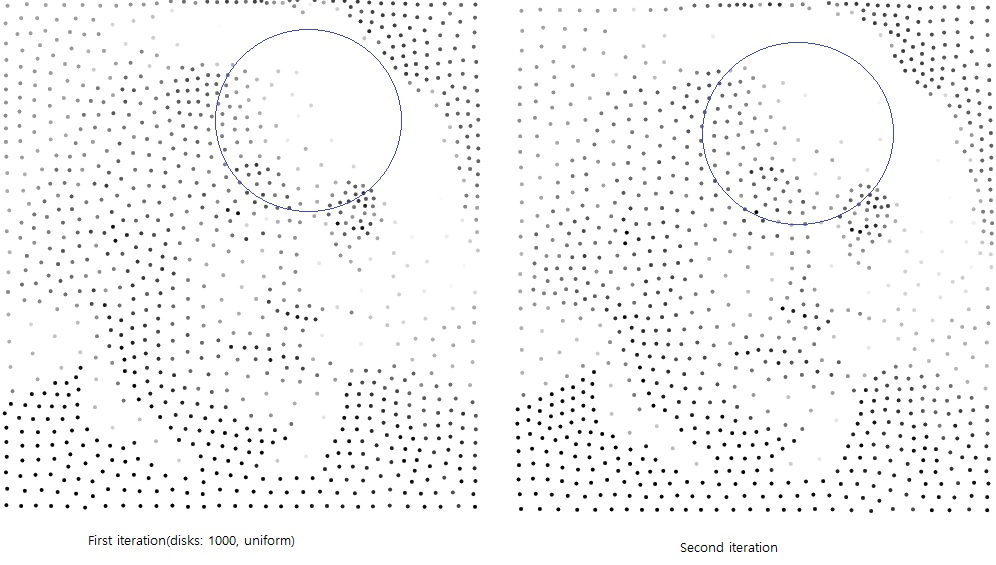
\includegraphics[width=80mm]{compare1.jpg}
  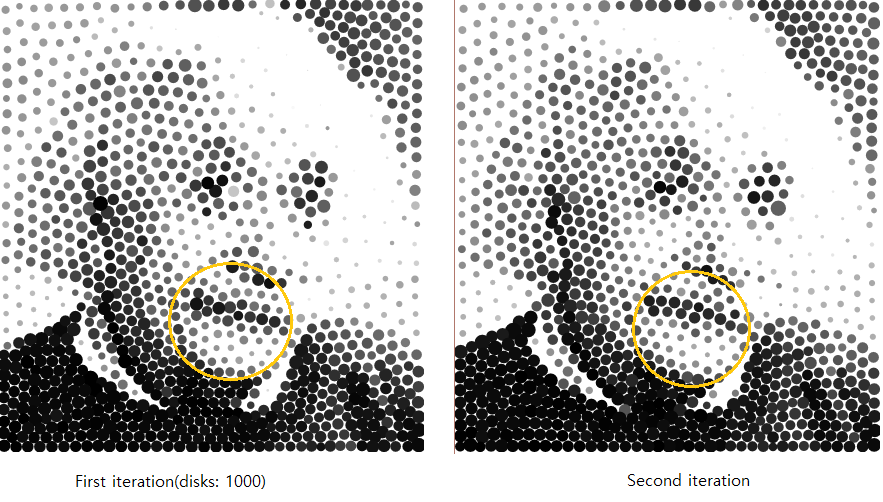
\includegraphics[width=80mm]{compare1(vor).jpg}
  \caption{Different locations of sample points for every iteration}  \label{compare1h}
\end{figure}


\textbf{2.If you vary the number of the disks in the output images, do these implementations produce the same distribution in the final image?}\\
Yes. I think so.\\
Since the distributions are affected by probability, in the assumption that we always have large number of sites, the set of sampled points is composed of more black points than white points. Therefore, the locations of the points will not vary much depending on the number of the disks, if the number of disks are large enough. If the number of the disks is relatively small to its image size, the distributions of the image maybe different.\\

\smallskip
\begin{figure}[hc]
  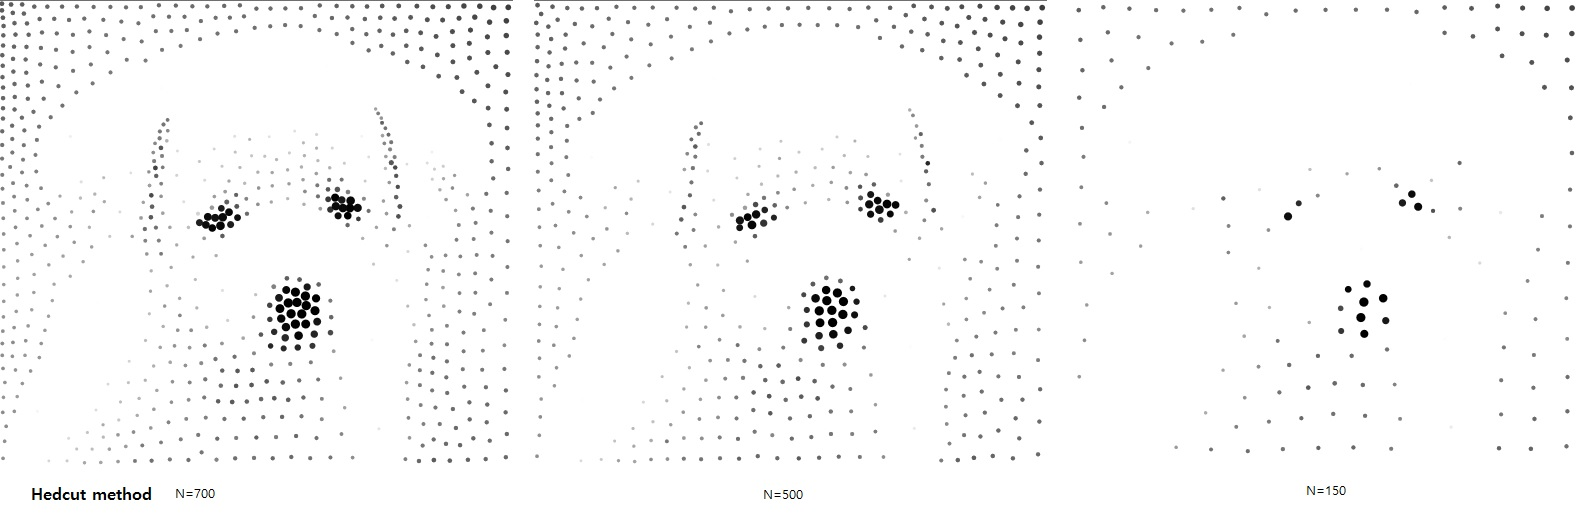
\includegraphics[width=83mm]{compare2.jpg}
  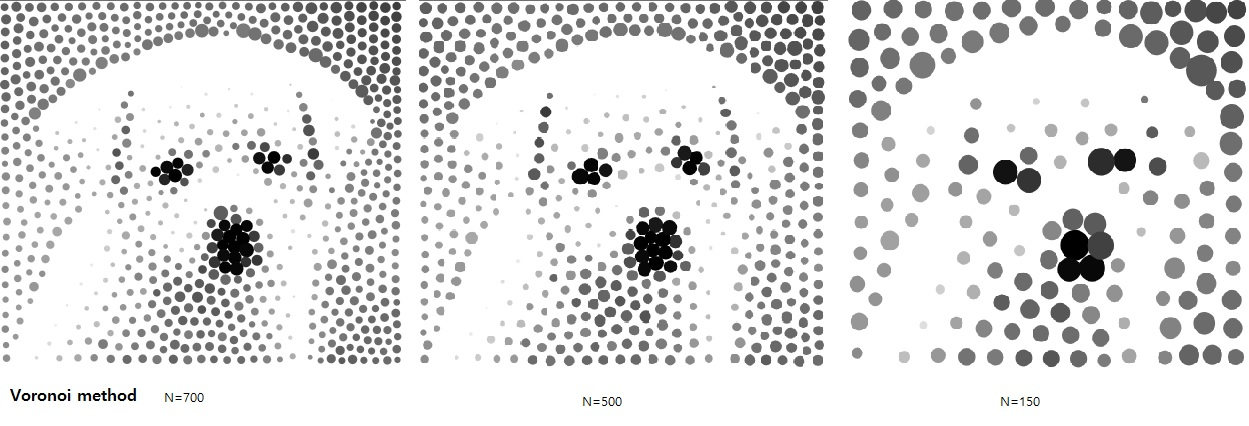
\includegraphics[width=80mm]{compare2(vor).jpg}
  \caption{Similar distributions of sample points}  \label{compare1h}
\end{figure}


\textbf{3.If you vary the number of the disks in the output images, is a method faster?}\\
Yes or No.\\
\begin{table}[ht]
\begin{tabular}{c c c}
\hline
 N(number of sites) & Hedcut & Voronoi \\ [0.5ex]
\hline
  50   & 14     & 50.38 \\
  100  & $\infty$ & 20.18sec \\
  1000 & $\infty$ & 16.26sec \\
  2000 & $\infty$ & 12.05sec \\
\hline
\end{tabular}
\end{table}
In using $[Hedcut]$ method, there are some points which oscillate. Because of that points the time, measured is infinity. But actually around 20sec after, all the cells stop(Fig.1).
I thought the answer will be positive. but it seems not for $[Hedcut]$ method. The speed of the stippling depends on the functions such as (1) computing voronoi diagram, (2) computing CVT, (3) moving sites.  But in  $[Voronoi]$ method, I can see the faster speed when I increased the number of sites. As the number of points increase, the image will be full of dense cells. Therefore the movement of sites will getting smaller so the termination point will be advanced.\\

\smallskip
\begin{figure}
\center
  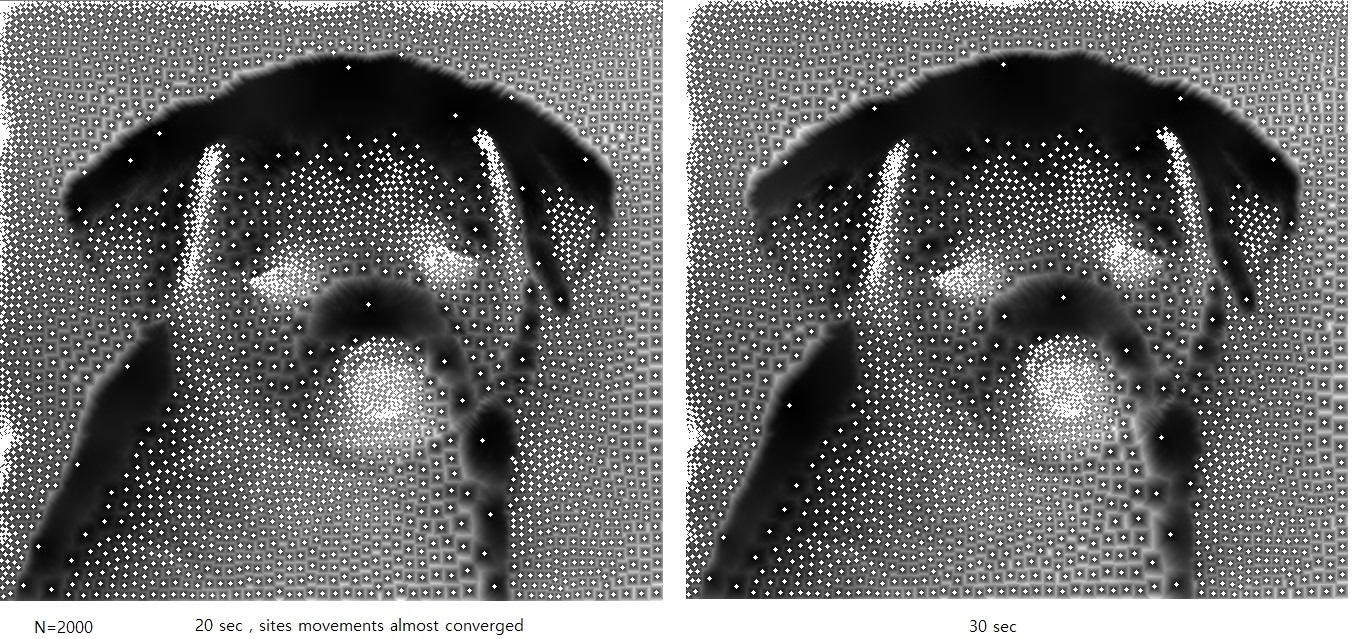
\includegraphics[width=80mm]{compare3(h).jpg}
  \caption{Most of the sites movements converge in Hedcut method }  \label{compare1h}
\end{figure}

\textbf{4.Does the pixel size, image brightness or contrast of image increase or decrease their difference?}\\
Yes. In most cases.\\
As we can see the Fig.2, the bigger pixel size the similarity decreases. One side the answer can be yes, and the other case it can be no. The image brightness is not the critical one if the feature of an image is centered, then the brightness of the picture does not matter. But if the most of area are bright then since both method picks points in the darker area, the result of stippling may lost the feature of image.(Fig.4) \\
In the second block picture we can compare the stippling result of GPU method to others. To produce a good stipping image, naturally we need many number of points to stipple. But under the same condition, the GPU method gives the best result to us. In the picture the partition between an object and background is more clear in GPU approach image.(Fig.5)

\begin{figure}[h]
\center
  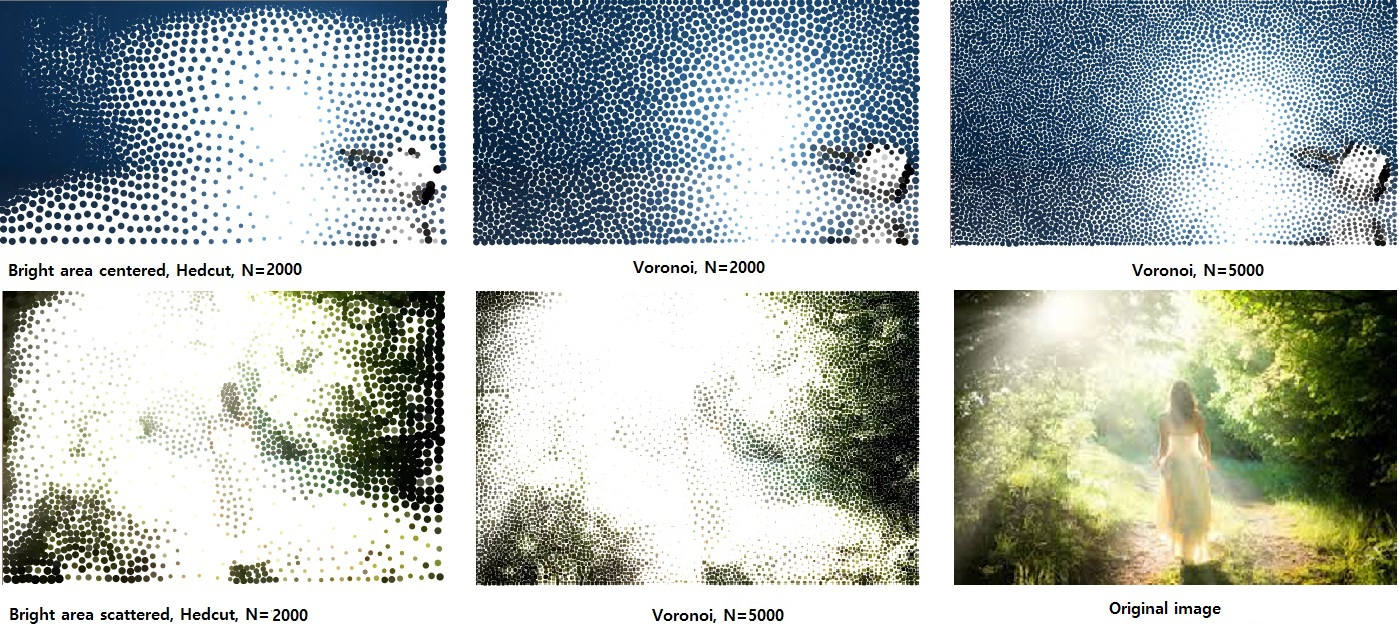
\includegraphics[width=140mm]{compare4.jpg}
  \caption{above. $[Voronoi]$ method approxmiate the feature well. below. both method doesn't work well}\label{compare1h}
  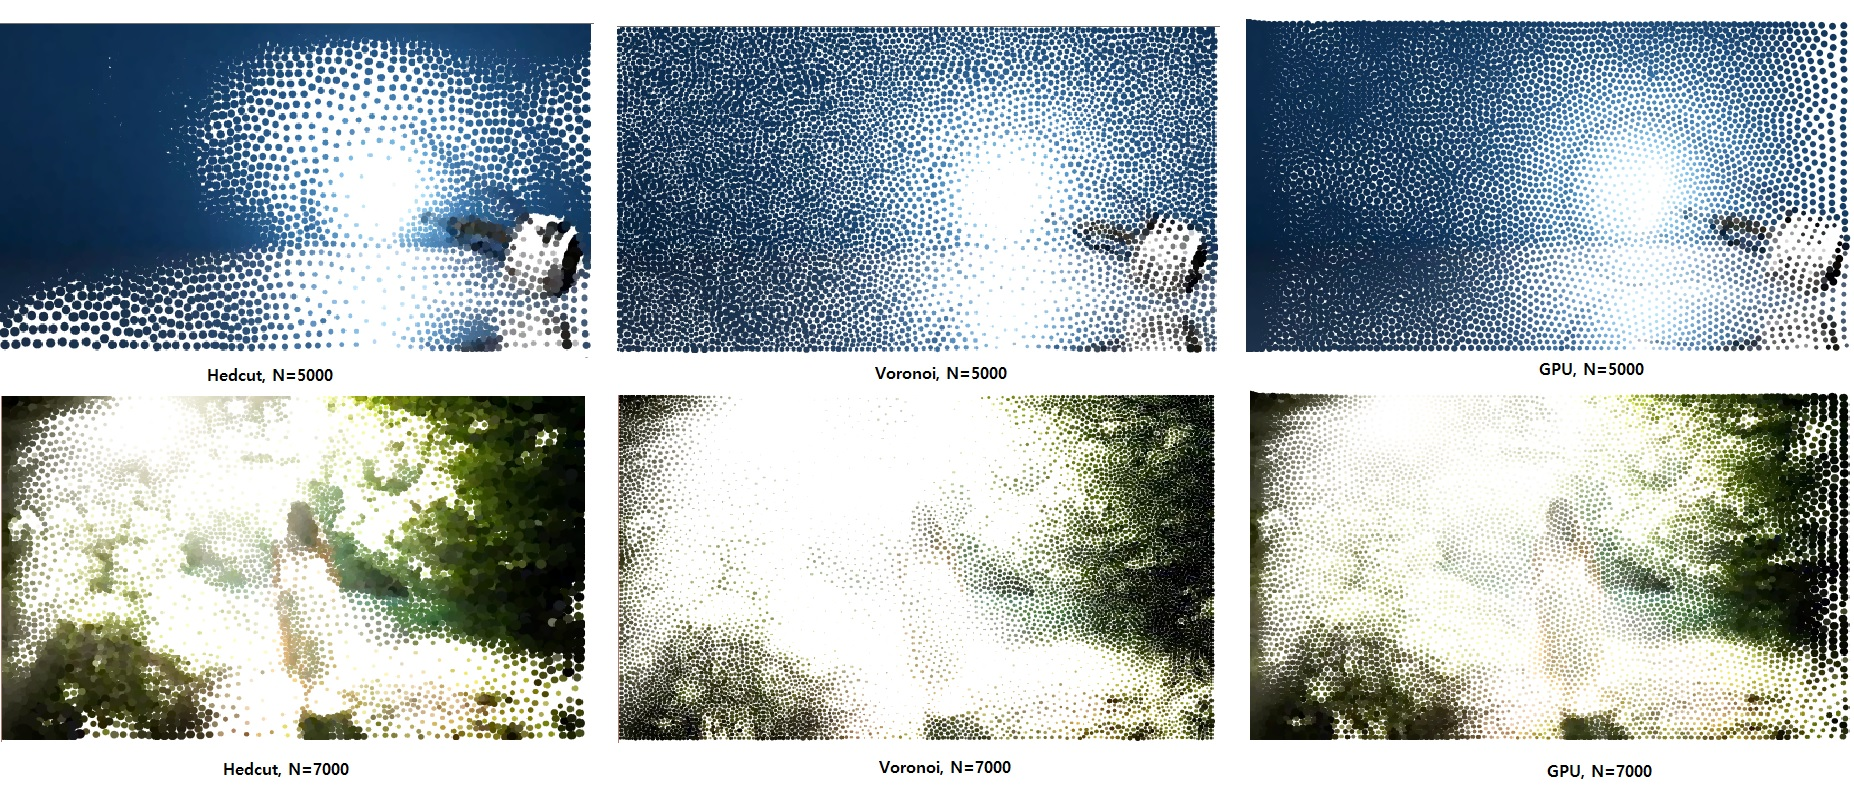
\includegraphics[width=140mm]{compare4(2).jpg}
  \caption{Compare with GPU based method}\label{GPU1}
\end{figure}

\bigskip
\textbf{5.Does the type of the image increase or decrease their difference?}\\
No.\\ For the hedcut method, the rate of similarity to original picture depends on whether the feature(darker side) of the image situated on the central of the picture. As we can see the above picture, the dispersion of (strong) lights or shiny reflection decreases the similarity of picture.\\

\textbf{6.Are the outputs of these stippling methods different the hedcut images created by artist?}
Not much.\\
As I increase the number of sample points, I get more natrual stippling image, closer to which, created by an artist.
\begin{figure}[h]
\center
  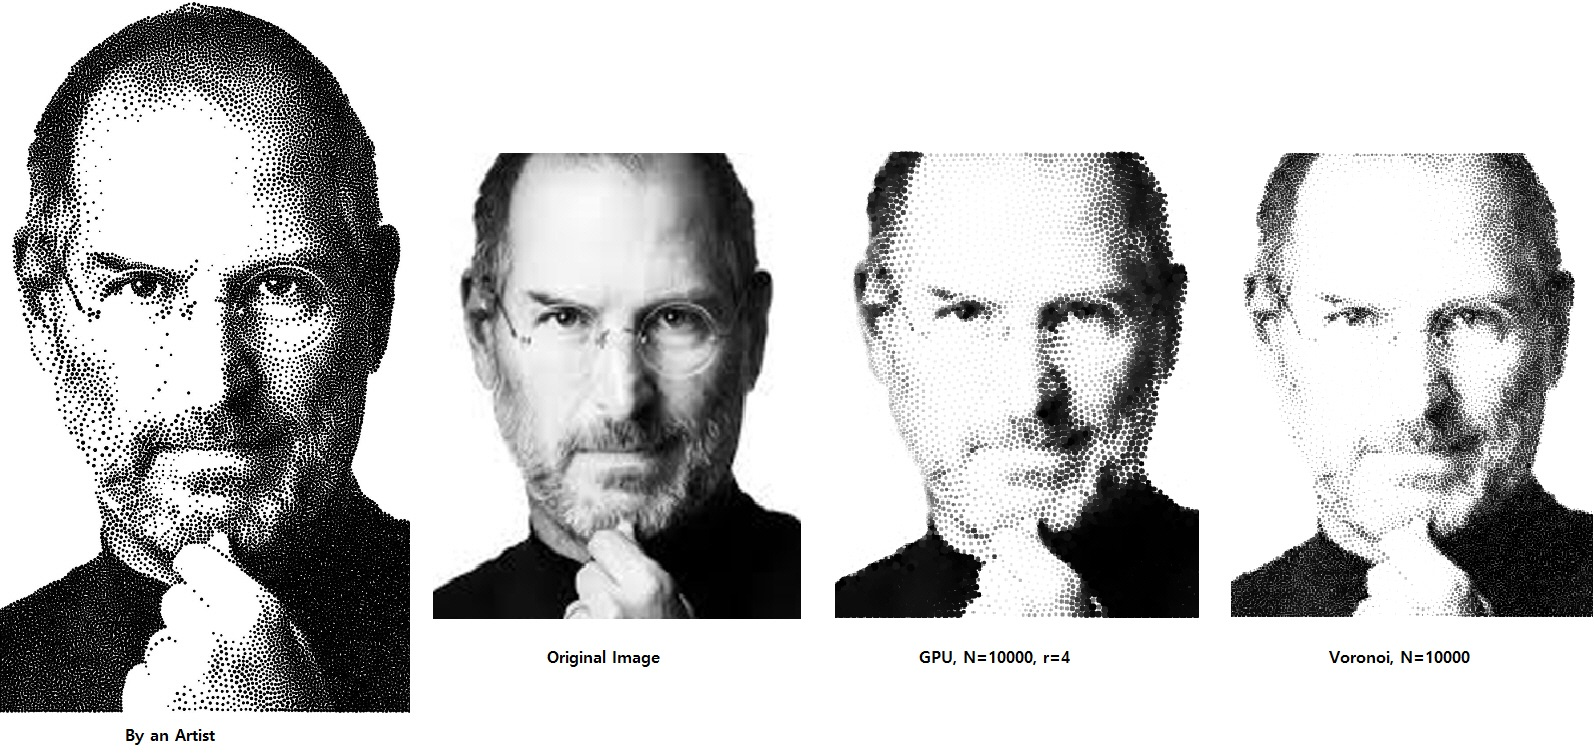
\includegraphics[width=160mm]{compare(art).jpg}
  \caption{Answer to question \#6 in part 2}\label{compare1h}
\end{figure}

\textbf{7.Does the difference in subpixel generates difference in resolution?}\\
It seems not at least in $[Voronoi]$ case. In using the bigger values of subpixel, the calculation time takes much longer but I can not see any improvement in resolution.(Fig.7)
\begin{figure}[h]
\center
  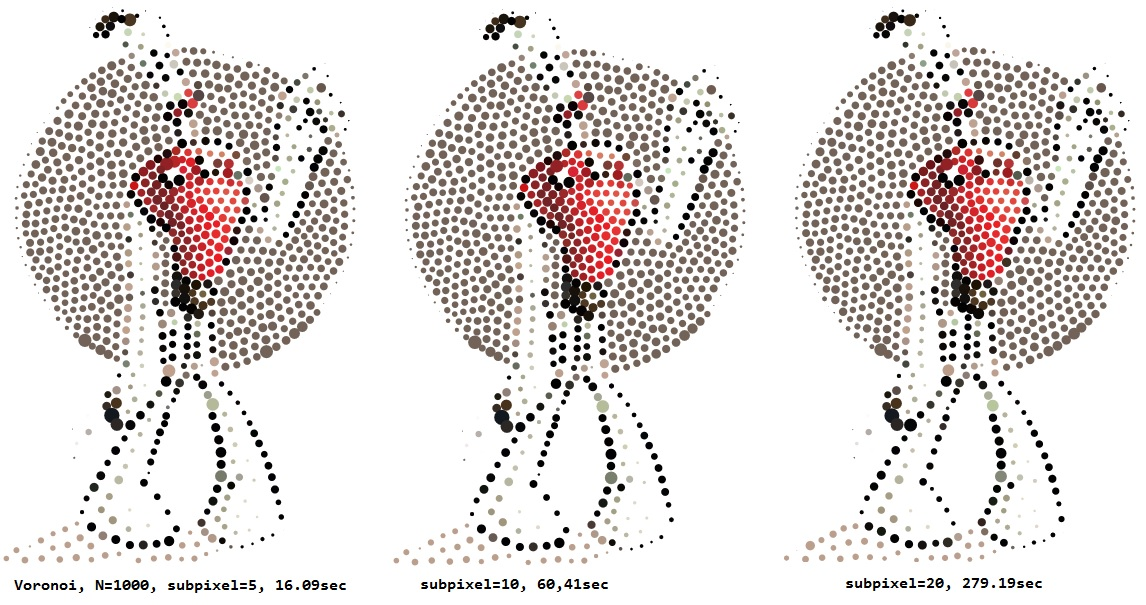
\includegraphics[width=160mm]{subpixel.jpg}
  \caption{Not much relativity between the different value of subpixels with the resolution}\label{compare1h}
\end{figure}

\section{Improvement of hedcuter method}
\textbf{1.Increased Computation Efficiency via GPU}\\
In GPU approach, drawing cones for each site is equivalent to calculating a voronoi diagram. Since we need to move every site to centroid of cells for the next iteration we need to store color information of each cell  therefore, we need N(number of sites) number of different colors. To generate arbitrary N number of colors, I used modulo concept. In this case we can generate at most $2^{24}$ number of color.(i.e. number of sites). Absolutely, using GPU we can make the program run faster.\\


\textbf{2.Natural Distribution\\}
To give weights to each radius of a cone, I used the intensity value which is calculated from the $[color2dist]$. For a point which has brighter color, it should have bigger radius than the darker one. So I computed the radius of each cone like this $[glutSolidCone(max$\_$radius*((2 - d)+0.5f*(1+d)), 1, 16, 1);]$. Since it is coarse the CVT using this GPU method is not exact. However, the stippling result of an image is quite satisfactory since the points are evenly distributed. (Fig.8,9)
\begin{figure}[h]
  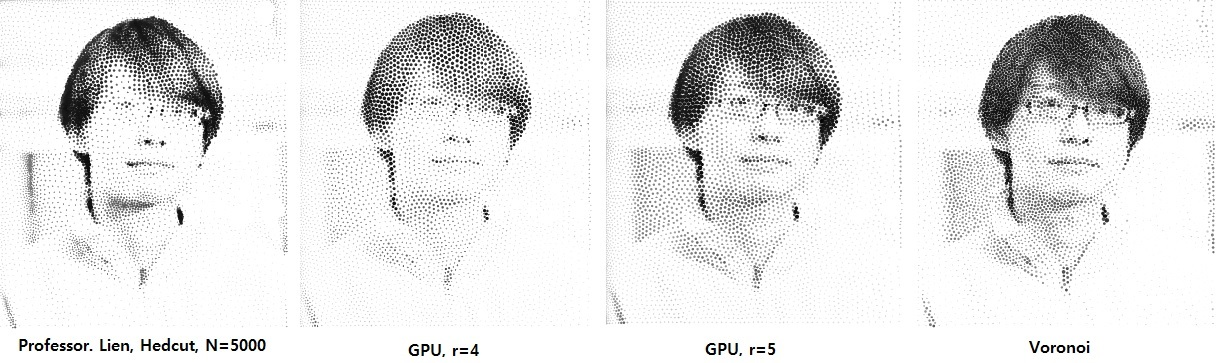
\includegraphics[width=160mm]{compare(prof).jpg}
  \caption{Improvement of Hedcut: Even distribution}\label{compare1h}
\end{figure}

\begin{figure}[h]
\center
  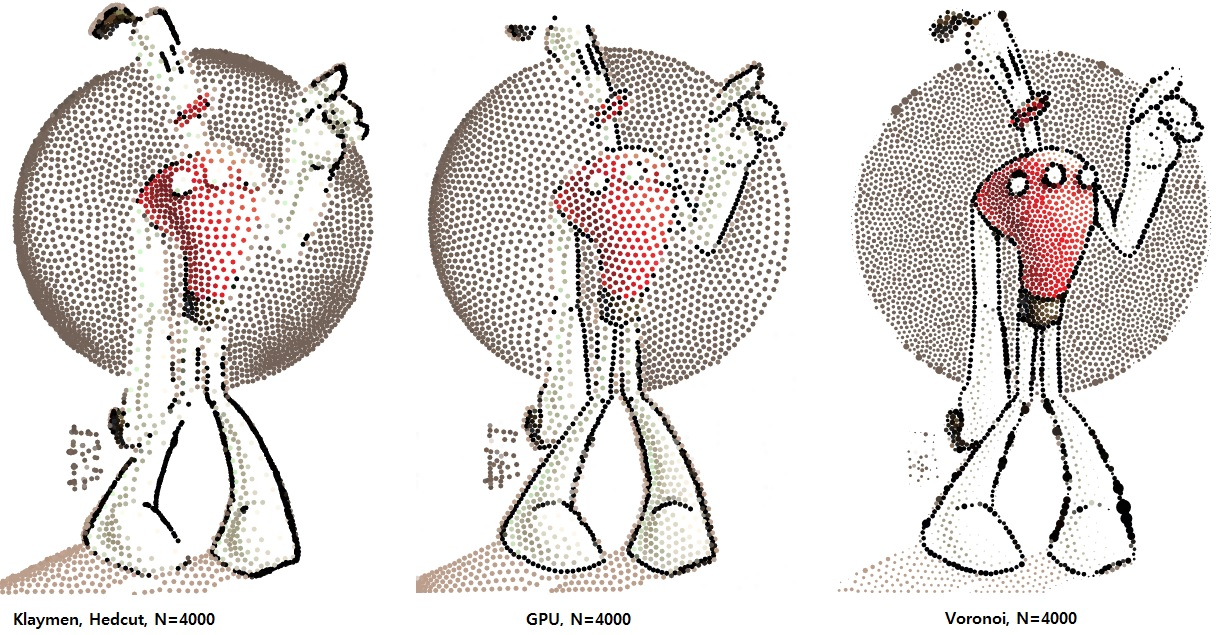
\includegraphics[width=160mm]{compare3(3).jpg}
  \caption{Improvement of Hedcut: Even distribution}\label{compare1h}
 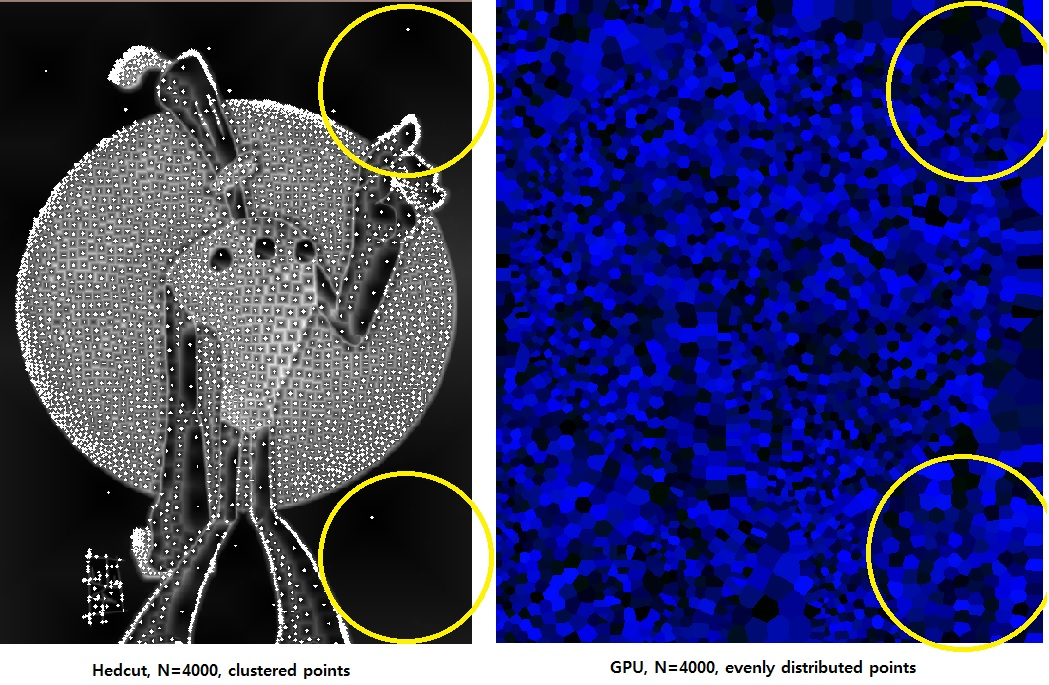
\includegraphics[width=160mm]{compare3(3-2).jpg}
  \caption{Improvement of Hedcut: Even distribution of cells}\label{GPU1}
\end{figure}

\textbf{3.Magnify the region of a brighter cell}\\
The probability is reversed. Was this intended? (Fig.11)
\begin{figure}[h]
\center
  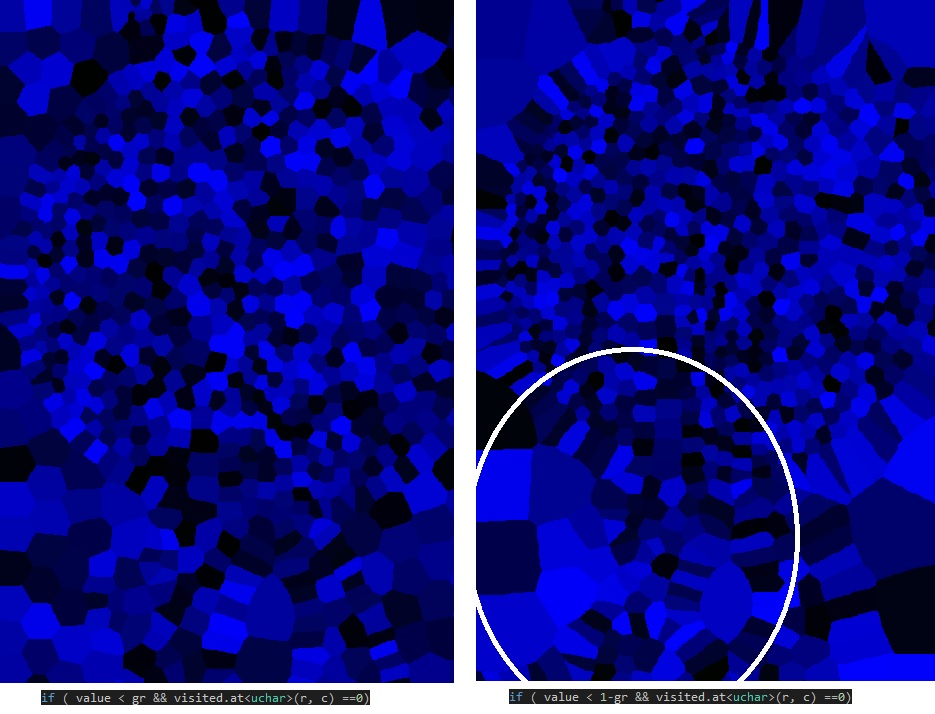
\includegraphics[width=140mm]{improvement4.jpg}
  \caption{The difference in cell movements. changed to 1-gr(right)}\label{compare1h}
\end{figure}

\textbf{4.Colorful Disks}\\
I include here some stippling pictures with color.
\begin{figure}[ht]
  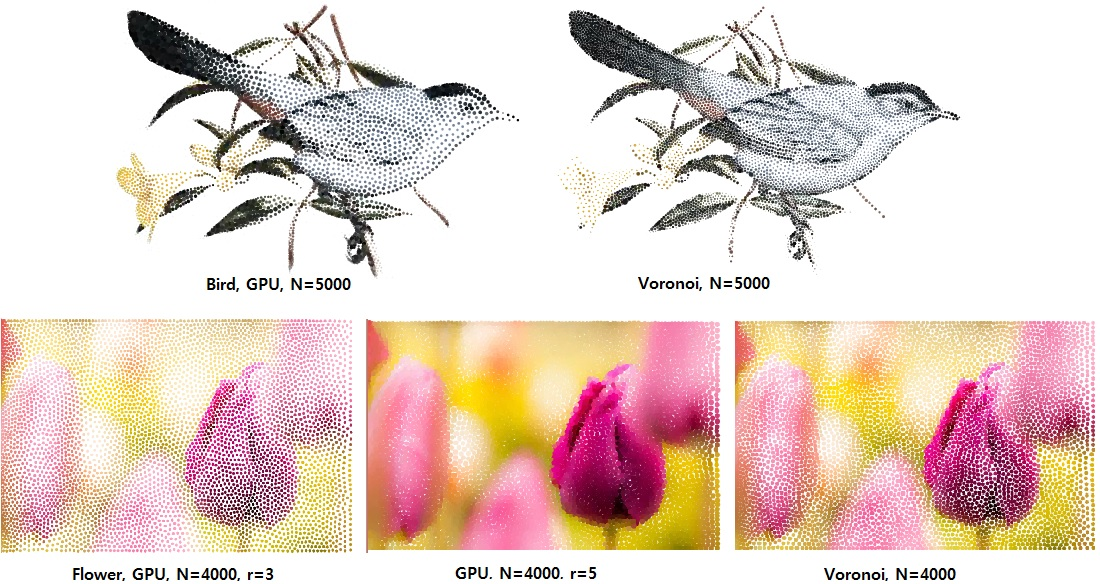
\includegraphics[width=160mm]{compare3(col).jpg}
  \caption{Compare GPU and Voronoi}\label{compare1h}
\end{figure}

\section{Conclusion}
In using GPU, the stippling result of images are quite satisfactory since the results are very similar to that of $[Voronoi]$'s. However, I could not shake off the doubt, the $[GPU]$ method inaccuately calculates CVT. Or It is my mistake, the results of $[GPU]$ method is different from the $[Hedcut]$. I only changed the code to draw cones in OpenGL so I expected only the improvement in the speed but luckily..? there is also improvement in the distributions. Maybe the difference is resulted from  $[glutSolidCone(max$\_$radius*((2 - d)+0.5f*(1+d)), 1, 16, 1);]$ this term which I thought this is a mild way to compute CVT.

\bibliographystyle{plain}
\bibliography{report}


\end{document}


